\section{Uživatelské případy}\label{sec:uzivatelskePripady}

Uživatelské případy blíže rozvádějí funkční požadavky (viz sekce~\ref{sec:seznamFunkčníchPožadavků}) a přesněji tak vymezují funkčnosti aplikace.
V rámci navrhovaného prototyp této aplikaci nejsou rozlišovány žádné uživatelské role.
Rozlišován je pouze přihlášený uživatel od obecného nepřihlášeného uživatele.
Z tohoto důvod se v uživatelských případech vyskytují pouze tito dva aktéři.

\begin{figure}[ht!]
    \centering
    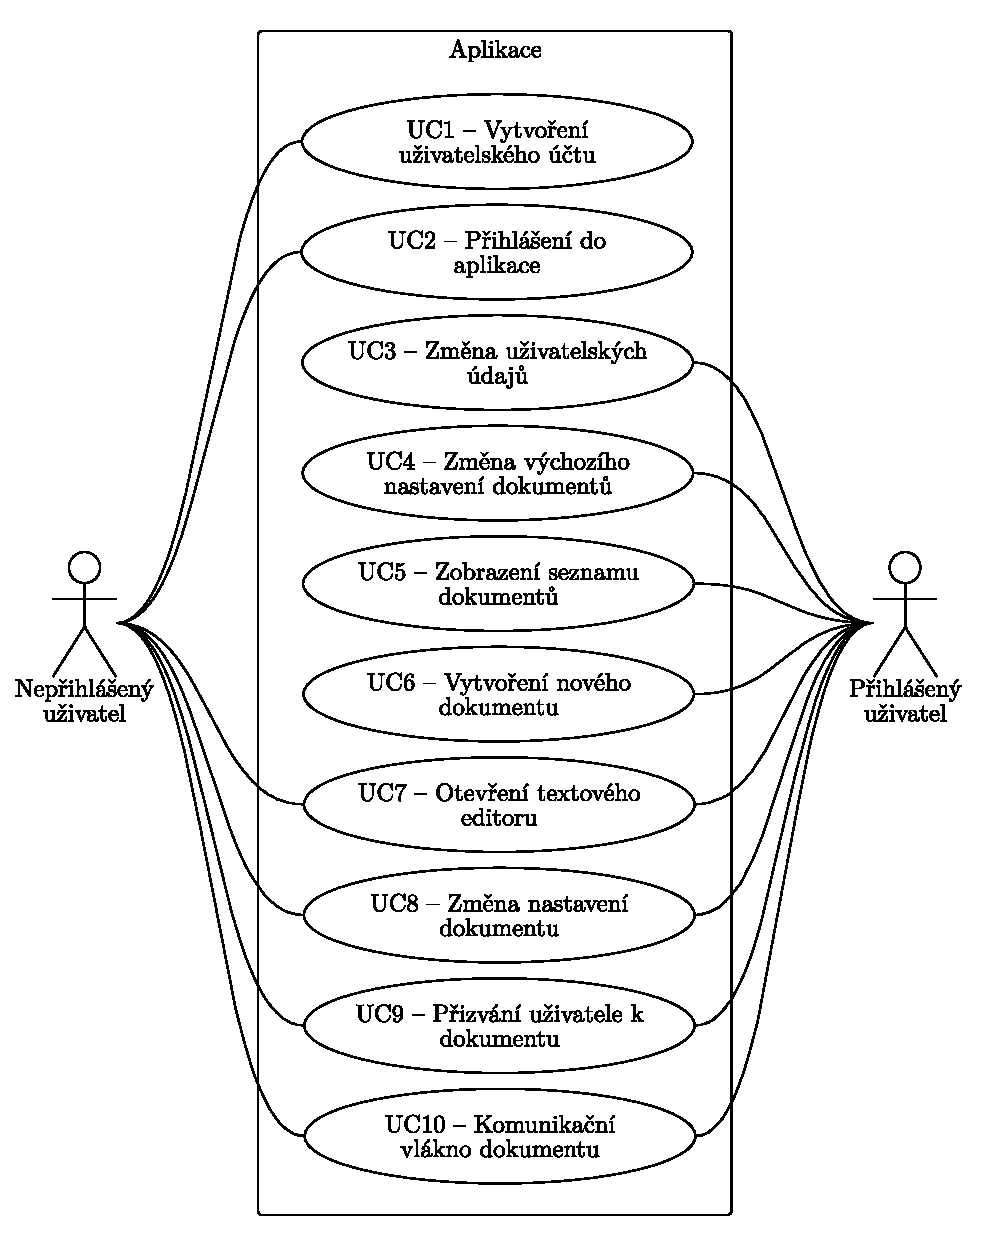
\includegraphics[width=0.9\textwidth]{partials/analyza/useCases.pdf}
    \caption{Diagram uživatelských případů}\label{fig:useCases}
\end{figure}


\paragraph{UC1 -- Vytvoření uživatelského účtu}

Nový nepřihlášený uživatel si může pomocí registračního formuláře vytvořit uživatelský účet.

Aplikace zobrazí registrační formulář, který obsahuje vstupní pole uživatelské jméno, email a heslo.
Uživatel formulář vyplní a odešle.
Aplikace formulář zpracuje (vytvoří nového uživatele se zadanými údaji) a uživatele přihlásí.
Uživateli je po přihlášení zobrazen seznam dokumentů (nyní prázdný) s tlačítkem vytvořit dokument.

\paragraph{UC2 -- Přihlášení do aplikace}

Uživatel, který si již vytvořil uživatelský účet se může k tomuto účtu kdykoliv přihlásit.

Nepřihlášenému uživateli je v horní liště aplikace k dispozici tlačítko \texttt{Při\-hlásit se}.
Po kliknutí na tlačítko je uživateli zobrazen přihlašovací formulář obsahující pole uživatelské jméno a heslo.
Uživatel je po vyplnění správných údajů a odeslání formuláře přihlášen.
Uživateli je po přihlášení zobrazen seznam dokumentů.

\paragraph{UC3 -- Změna uživatelských údajů}

Přihlášený uživatel může kdykoliv provést změnu svých přihlašovacích údajů.

Přihlášený uživatel má v horní liště zobrazené tlačítko \texttt{Nastavení}.
Po kliknutí na toto tlačítko je uživateli zobrazen formulář pro změnu údajů.
Formulář obsahuje pole uživatelské jméno, email, nové heslo a aktuální heslo.
Uživatel vyplní údaje, které chce změnit a aktuální heslo.
Aplikace po odeslání zobrazí informaci o úspěšné změně údajů.

\paragraph{UC4 -- Změna výchozího nastavení dokumentů}

Přihlášený uživatel může změnit výchozí nastavení dokumentů.
Toto nastavení je následně aplikováno na uživatelem nově vytvořené dokumenty (u již existujících dokumentů se změny neprojeví).

Přihlášený uživatel má v horní liště zobrazené tlačítko \texttt{Nastavení}.
Po kliknutí na toto tlačítko je uživateli zobrazen panel s tlačítkem \texttt{Nastavení dokumentů}, který se nachází nad formulář pro změnu uživatelských údajů.
Kliknutím na tlačítko je uživateli zobrazen formulář pro změnu výchozího nastavení dokumentů.
Uživatel upraví pole, které chce změnit, a formulář odešle.
Aplikace po odeslání zobrazí informaci o úspěšné změně nastavení.

\paragraph{UC5 -- Zobrazení seznamu dokumentů}

Přihlášený uživatel si může zobrazit seznam jím vytvořených dokumentů, seznam dokumentů ke kterým byl přizván a seznam v minulosti otevřených dokumentů.

Přihlášený uživatel má v menu aplikace k dispozici tlačítka \texttt{Mé dokumenty}, \texttt{Sdílené} a \texttt{Poslední}.
Po kliknutí na tlačítko aplikace zobrazí korespondující seznam dokumentů.

\paragraph{UC6 -- Vytvoření nového dokumentu}

Přihlášený uživatel může kdykoliv vytvořit nový dokument.
Počet vytvořených dokumentů není nijak omezený.

Přihlášený uživatel má k dispozici v horní liště tlačítko \texttt{Vytvořit nový dokument}.
Po kliknutí na tlačítko aplikace dokument vytvoří a aplikuje na něj uživatelovo výchozí nastavení pro dokumenty.
Uživatel je přesměrován do textového editoru nově vytvořeného dokumentu.

\paragraph{UC7 -- Otevření textového editoru}

Uživatel může přistoupit přímo k veřejnému odkazu dokumentu nebo otevřít editor kliknutím na odkaz v seznamu dokumentů.
Po otevření editoru je uživateli zobrazen samotný textový editor a uživatel může začít dokument upravovat (pokud k tomu má pro daný dokument dostatečné oprávnění).

\paragraph{UC8 -- Změna nastavení dokumentu}

Uživatel může změnit nastavení dokumentu přímo z textového editoru (pokud k tomu má pro daný dokument dostatečná oprávnění).
Aplikace zobrazí nad editorem tlačítko s ikonou ozubeného kola, které po kliknutí otevře panel s jednotlivými poli nastavení.

Nastavení je na editor a dokument aplikováno ve skutečném čase všem upravujícím uživatelům.

\paragraph{UC9 -- Přizvání uživatele k dokumentu}

Uživatel může přizvat ostatní uživatele ke spolupráci nad dokumentem a to přímo z textového editoru (pokud k tomu má pro daný dokument dostatečná oprávnění).
Aplikace zobrazí nad editorem tlačítko \texttt{Sdílet}, které po kliknutí otevře panel s možnostmi sdílení dokumentu.

Uživatel může změnit výchozí práva pro příchozí uživatele pomocí veřejného odkazu a následně odkaz sdílet.
Nastavení práv veřejného odkazu se objeví po kliknutí na ikonu ozubeného kola, která se nachází vedle pole s veřejným odkazem.
Po odeslání aplikace nastavení uloží a zobrazí potvrzení.

Uživatel také může přizvat jednotlivé uživatele kliknutím na tlačítko \texttt{Nová pozvánka}.
Po kliknutí na toto tlačítko aplikace zobrazí formulář pro vytvoření pozvánky s poli uživatelské jméno a oprávnění.
Uživatel pole vyplní podle potřeby a formulář odešle.
Aplikace po odeslání vyhledá uživatele podle uživatelského jména a v případě nalezení vytvoří pozvánku k dokumentu.
Aplikace následně obnoví seznam pozvánek pod formulářem a zobrazí informaci o úspěchu, či neúspěchu pozvání.

\paragraph{UC10 -- Komunikační vlákno dokumentu}

Uživatel může přispívat do komunikačního vlákna přímo z textového editoru (pokud k tomu má dostatečná oprávnění).
Panel s komunikačním vláknem je zobrazen po kliknutí na tlačítko s ikonou konverzační bubliny.

\subsection{Matice pokrytí funkčních požadavků}\label{subsec:maticePokrytíFunkčníchPožadavků}

Při návrhu uživatelských případů je důležité ověřit, zda-li jsme případy pokryli všechny funkční požadavky.
Právě k tomuto účelu slouží matice pokrytí funkčních požadavků (viz tabulka~\ref{tab:maticePokryti}).
Matice pokrytí nám ukazuje, které funkční požadavky jsou pokryt v rámci jednotlivých uživatelských případů.

\begin{table}[ht!]
    \centering
    \caption{Matice pokrytí uživatelských požadavků}\label{tab:maticePokryti}

    \begin{tabular}{r|c c c c c c c c c c}
           & UC1      & UC2      & UC3      & UC4      & UC5      & UC6      & UC7      & UC8      & UC9      & UC10     \\ \hline
        F1 & $\times$ & $\times$ & $\times$ & $\times$ &          &          &          &          &          &          \\
        F2 &          &          &          & $\times$ & $\times$ & $\times$ & $\times$ &          & $\times$ &          \\
        F3 &          &          &          &          &          &          & $\times$ & $\times$ & $\times$ & $\times$ \\
    \end{tabular}
\end{table}
